%{ 
% This opens a block comment for MATLAB and Octave
\documentclass{article}

\usepackage[margin=3cm]{geometry}
\usepackage{verbatim}
\usepackage{graphicx}
\usepackage{natbib}
\usepackage{times}
\usepackage{footnote}
\usepackage[utf8]{inputenc}
%\usepackage[sort&compress,square,comma,authoryear]{natbib}


\newenvironment{matlab}{\comment}{\endcomment}
\newenvironment{octave}{\comment}{\endcomment}
\newenvironment{matlabv}{\verbatim}{\endverbatim}
\newenvironment{octavev}{\verbatim}{\endverbatim}

% Para incluir código Matlab/Octave añadir un chunk de código 
\begin{matlab}
%}
% El código Matlab/Octave comienza aquí
% Se inicia el código añadiendo una semilla para el generador de números aleatorios.
% Se limpia la memoria de variables y figuras.
% Se sugiere definir aquí cualquier variable que quiera utilizarse de forma global.
% Se pueden definir también aspectos estéticos como tamaños de fuentes,
% rutas a ficheros scripts, etc.

% Limpiar variables y borrar figuras
clear all
close all

% Definir semillas del generador de números aleatorios.
rand('seed', 1e5);
randn('seed', 1e5);

% Definir tipo y tamaño de fuentes.
fontName = 'times';
fontSize = 26;

% Obtener la version de MATLAB/Octave
a = ver('octave');
if length(a) == 0
  a = ver('matlab');
end
fid = fopen('vers.tex', 'w');
fprintf(fid, [a.Name ' version ' a.Version]);
fclose(fid);

% Obtener la arquitectura del sistema.
fid = fopen('computer.tex', 'w');
fprintf(fid, ['\\verb+' computer '+']);
fclose(fid);

% Obtener fecha.
fid = fopen('date.tex', 'w');
fprintf(fid, datestr(now, 'dd/mm/yyyy'));
fclose(fid);

%{
\end{matlab}


\title{MATweave: Integración de código MATLAB/Octave en \LaTeX \footnote{Adaptado de  Neil D. Lawrence}}
\author{Mario Mañana Canteli \\\texttt{mananam@unican.es}\\Dpto. de Ingeniería Eléctrica y Energética\\Universidad de Cantabria}
\date{18/01/2018} % Gives date when code was run.
\begin{document}

\maketitle


\begin{abstract}
MATweave define un procedimiento para integrar código MATLAB/Octave dentro de documentos \LaTeX. El objetivo final es facilitar a los usuarios de MATLAB/Octave la generación integral de investigación reproducible.
\end{abstract}

\section{Introducción}

MATweave proporciona un método simple para la generación de informes que integran datos y código utilizando \LaTeX\ como lenguaje de edición, y puede considerarse como un sistema básico para la generación de documentos basados en el paradigma de la investigación reproducible. El objetivo final de este conjunto de herramientas es obtener un entregable que integre documentación, datos y código que pueda, además, ser reutilizado por otros usuarios.
MATweave está inspirado en Sweave \cite{lmucs-papers:Leisch:2002}, diseñado originalmente para combinar programas en R y \LaTeX. 

\subsection{Procedimiento}

La idea que subyace detrás de MATweave es utilizar códigos específicos para indicar el inicio y fin del fragmento de código dentro del fichero \LaTeX.
\begin{enumerate}
\item El primer procedimiento es utilizar códigos de comentario tipo bloque, introducidos en Octave 3.2 and MATLAB R14.

Los comentarios tipo bloque en MATLAB/Octave se abren con \texttt{\%\{} y se cierran con \texttt{\%\}} permitiendo incluir código dentro:
\begin{verbatim} 
%{
Esto es un comentario!                         
%}                                         
for i = 1:10                               
  % Este codigo esta fuera del comentario.
  disp(i)                                  
end                                        
\end{verbatim}

El `truco' consiste en que un bloque de comentario en MATLAB/Octave es un comentario en \LaTeX (debido a que comienza con el carácter \texttt{\%}), pero  \emph{no} un bloque de comentario.
\begin{verbatim} 
%{
En MATLAB/Octave esto sería un comentario, pero en \LaTeX sí se compilaría.  
Esto significa que es posible escribir código \LaTeX, como por ejemplo 
$\tau = 2\pi$, dentro de un script MATLAB. 
Ahora debemos ser capaces de escribir MATLAB/Octave dentro de un 
fichero \LaTeX.
%}
\end{verbatim}

\item El segundo `truco' es incluir el paquete \texttt{verbatim} y utilizarlo para definir un nuevo entorno MATLAB/Octave utilizando los comandos siguientes:
\begin{verbatim}
\newenvironment{matlab}{\comment}{\endcomment}    
\newenvironment{octave}{\comment}{\endcomment}    
\newenvironment{matlabv}{\verbatim}{\endverbatim} 
\newenvironment{octavev}{\verbatim}{\endverbatim} 
\end{verbatim}


Esto permitirá incluir código MATLAB/Octave que no será leído por \LaTeX utilizando: \texttt{\textbackslash begin\{octave\}
    ... \textbackslash end\{octave\}}, así como código que será mostrado en un entorno verbatim utilizando \texttt{\textbackslash begin\{octavev\} ... \textbackslash end\{octavev\}}. Por supuesto es posible hacer esto mismo utilizando el entorno estándar \texttt{verbatim}. Sin embargo, utilizando un nuevo entorno es posible definir los fragmentos de código que se muestran y/o se ejecutan.
\end{enumerate}

\subsection{Ejemplo}

El código siguiente se ha desarrollado utilizando el entorno \texttt{matlabv} definido anteriormente. El código fuente de este documento comienza con un código de bloque abierto MATLAB/Octave \texttt{\%\{}. Dicho código se cierra al comiendo de un bloque MATLAB/Octave, de forma que será compilado por dichos programas.

\begin{matlabv}
%} 
% El codigo MATLAB/Octave comienza aqui
tau = 2*pi;
x = linspace(-3, 3, 100)';
y = 1/sqrt(tau)*exp(-0.5*x.^2);
plot(x, y, 'r-');
set(gca, 'fontname', fontName, 'fontsize', fontSize);
print -dpdf myGaussian.pdf
% El codigo MATLAB/Octave finaliza aqui
%{ 
\end{matlabv}

La combinación de dos bloques significa que el código fuente de este documento puede ser compilado en \LaTeX o en MATLAB/Octave.

\section{Ejecutando MATweave}

El procedimiento para generar el documento se resume a continuación:

\begin{itemize}
\item Ejecutar el comando `source fichero.tex' en Matlab/Octave.
\item Ejecutar el comando `pdflatex fichero.tex' en la línea de comandos del sistema operativo. Si el documento incluye referencias bibliográficas es necesario realizar una secuencia:
	\begin{itemize}
		\item `pdflatex fichero.tex'
		\item `bibtex fichero.tex'
		\item `pdflatex fichero.tex'
	\end{itemize}
\end{itemize}

Como se ha comentado, el fichero \LaTeX\ puede ser ejecutado en Octave con el comando \texttt{source}. Como ejercicio, guardar este documento como \texttt{myexample.tex} y ejecutar \texttt{source myexample.tex} en la línea de comandos de Octave. En MATLAB el procedimiento es un poco más complicado.

La salida del código incluye figuras en formato .pdf. La primera de las figuras se muestra en la Figura \ref{fig:one}.

\begin{figure}
\centerline{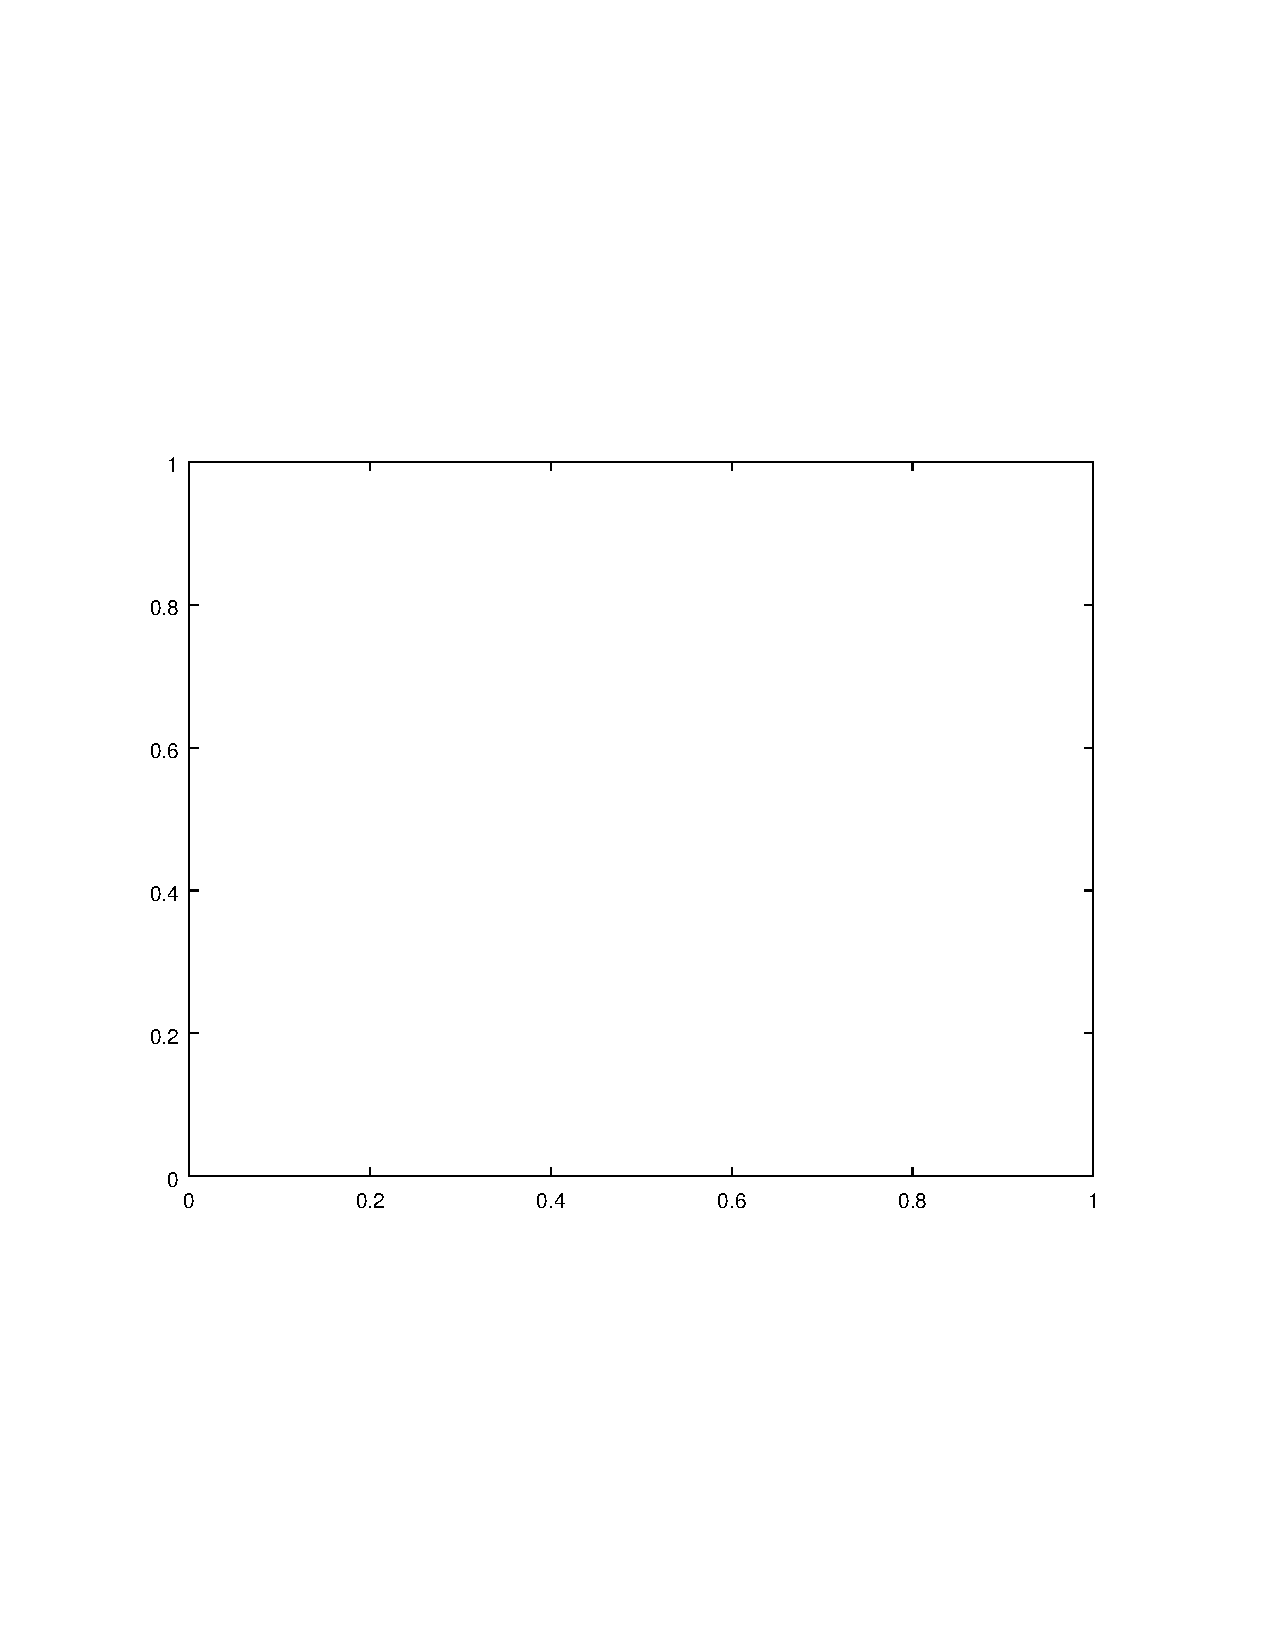
\includegraphics[width=0.5\textwidth]{myGaussian}}
\caption{Curva de densidad de probabilidad Gausiana.}\label{fig:one}
\end{figure}

El código MATLAB/Octave puede ser mostrado u ocultado en el documento según convenga en cada momento atendiendo a la necesidad de documentar un procedimiento de cálculo e incluso por motivaciones de depuración del código.
A modo de ejemplo, el histograma mostrado en la Figura \ref{fig:two}  ha sido codificado utilizando el entorno \texttt{\textbackslash begin\{matlab\} ... \textbackslash end\{matlab\}}.

\begin{matlab}
%}
a = randn(1000, 1);
hist(a, 30);
set(gca, 'fontname', fontName, 'fontsize', fontSize);
print -dpdf myHistogram.pdf
%{
\end{matlab}

\begin{figure}
\centerline{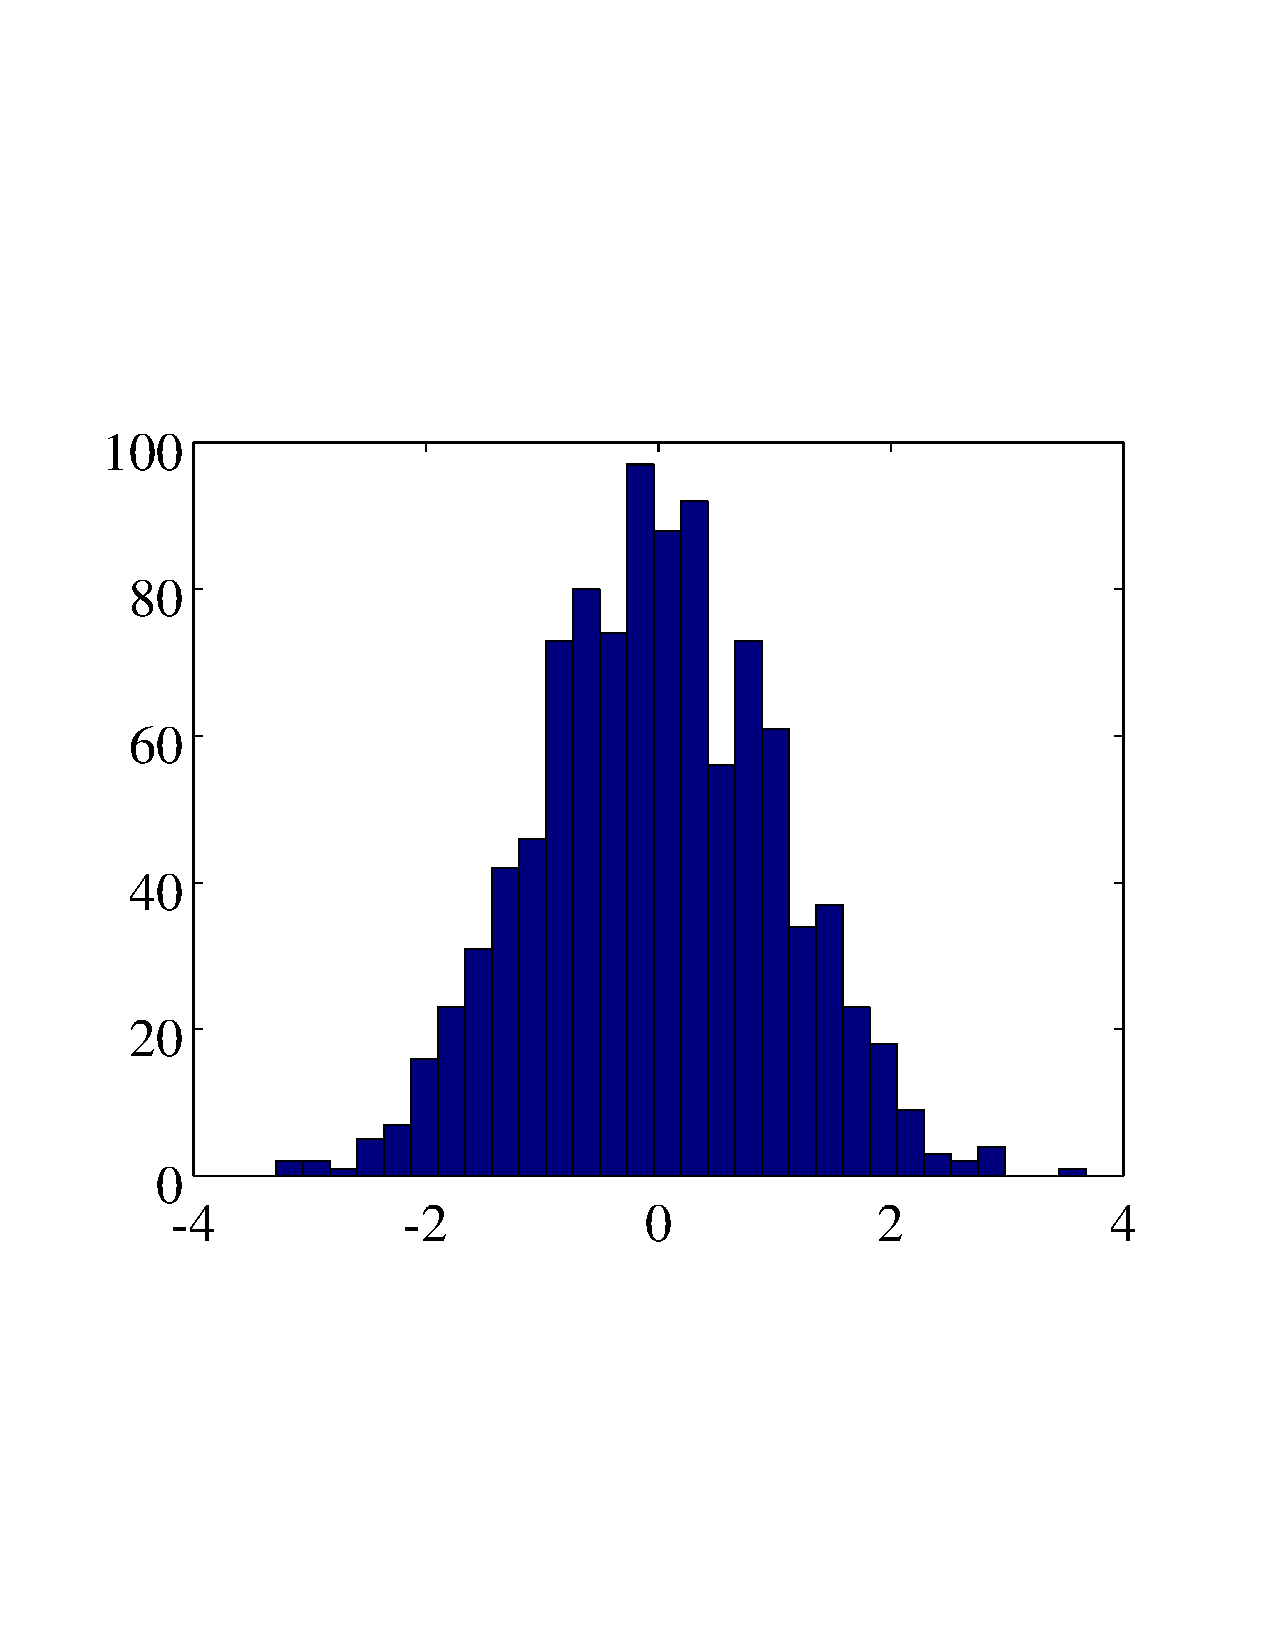
\includegraphics[width=0.5\textwidth]{myHistogram}}
\caption{Histograma con 1000 muestras de una distribución Gausiana.}\label{fig:two}
\end{figure}

Otra posibilidad que puede mejorar la visualización de código es utilizar el paquete \texttt{listings}. Otra posibilidad para mejorar la automatización del documento es utilizar MATLAB/Octave para generar un fichero .tex con la tabla que se pretenda visualizar en el documento \LaTeX.

\begin{matlabv}
%}
% Codigo para generar una tabla con numeros aleatorios.
rows = 3;
cols = 4;
numSigFigs = 3;
resultMatrix = randn(3, 4); 
fid = fopen('results.tex', 'w');
for i = 1:rows
  for j = 1:cols
    fprintf(fid, ['$' num2str(resultMatrix(i, j), numSigFigs) '$']);
    if j < cols
      fprintf(fid, ' & ');
    end
  end
  if i < rows
    fprintf(fid, '\\\\\n');
  end 
end
fclose(fid);
%{
\end{matlabv}

El fichero de resultados con la tabla puede ser incorporado al documento mediante el código \texttt{\textbackslash
  input\{results.tex\}} y mostrado como aparece en la Tabla \ref{table:one}.

\begin{table}
\caption{Ejemplo de una tabla de números aleatorios con MATLAB/Octave.}\label{table:one}
\begin{center}
\begin{tabular}{c|c|c|c}
$A$ & $B$ & $C$ & $D$ \\
\hline
$-0.442$ & $1.59$ & $0.302$ & $-1.5$\\
$-0.418$ & $2.39$ & $-0.123$ & $0.632$\\
$-1.46$ & $1.08$ & $0.128$ & $-2.35$
\end{tabular}
\end{center}
\end{table}

\subsection{Consejos adicionales}

Se considera una buena medida comenzar el fichero \LaTeX\ con un conjunto de comandos que limpien la memoria, definan las rutas necesarias, borren las figuras, etc.

\subsection{Nota para usuarios de Beamer}

Aquellos usuarios de MATweave que generen presentaciones utilizando Beamer deben utilizar la opción \texttt{[fragile]} 
en aquellas transparencias que contengan el entorno MATLAB/Octave. Sin dicha opción Beamer no será capaz de manejar los entornos \texttt{verbatim} o \texttt{comment}.

Se necesita una versión MATLAB R14 o superior y Octave 3.2 o superior.  Para compilar el fichero en Linux: 

\begin{verbatim}
octave --eval source\ myexample.tex
\end{verbatim}

o

\begin{verbatim}
matlab < myexample.tex
\end{verbatim}

y después,

\begin{verbatim}
pdflatex myexample
\end{verbatim}

\section{Conclusiones}

Se ha mostrado que la integración de código MATLAB/Octave con \LaTeX puede realizarse mediante procedimientos sencillos. El procedimiento no es tan elegante como la pareja Sweave con R, donde tanto las variables como las gráficas se integran en el texto de forma natural.

El objetivo de MATweave es facilitar la generación de documentos reproducibles.

\subsection*{Nota}

Este documento fue generado utilizado MATweav utilizando Octave version 4.0.0 en una máquina \verb+x86_64-pc-linux-gnu+. El documento fue generado el 18/01/2018.

\bibliographystyle{plain}
\bibliography{myexample}

\end{document}
%} 
% No olvidar el final del comentario MATLAB al final del fichero!
